\documentclass{article}

\usepackage{hw}
\usepackage{bm}
\usepackage{amsmath}
\usepackage{graphicx}
\usepackage[colorlinks=true,urlcolor=blue]{hyperref}
\usepackage{geometry}
\geometry{margin=1in}
\usepackage{multicol}
\usepackage{paralist}
\usepackage{todonotes}
\setlength{\marginparwidth}{2.15cm}
\usepackage{booktabs}
\usepackage{enumitem}

% Some commands to allow solutions to be embedded in the assignment file.
\ifcsname issoln\endcsname \else \def\issoln{0} \fi
\newcommand{\soln}[1]
{
  \if\issoln 1
  \textbf{Solution:}
  #1
  \fi
}

\begin{document}

\section*{}
\begin{center}
  \centerline{\textsc{\LARGE Homework 1{\if\issoln 1 Solutions \else \fi}}}
  \vspace{0.5em}
  \centerline{\textsc{\Large Naive Bayes and Logistic Regression}}
  \vspace{1em}
  \textsc{\large CMU 10-701: Machine Learning (Fall 2014)} \\
  \url{https://piazza.com/cmu/fall2014/1070115781/home}
  \centerline{OUT: Sept 12, 2014}
  \centerline{DUE: Sept 25, 2014, 11:59 PM}
\end{center}

\if\issoln 1 \else
\section*{START HERE: Instructions}

\begin{itemize*}


\item \textbf{Late days:} The homework is due Thursday September 25th, at 11:59PM. You have five late days to use throughout the semester, and may use at most three late days on any one assignment. Once the allowed late days are used up, each additional day (or part of a day) will subtract 1 from the normalized score for the assignment. View the full late days policy on \href{https://piazza.com/class/hxwaa1bxuze4xj?cid=10}{Piazza}.

\item \textbf{Collaboration policy:} Collaboration on solving the homework is allowed, after you have thought about the problems on your own.  It is also OK to get inspiration (but not solutions) from books or online resources, again after you have thought about the problems on your own.  There are two requirements: first, cite your collaborators and resources fully and completely (e.g., ``Jane explained to me what is asked in Question 3.4'' or ``I found an explanation of conditional independence on page 17 of Mitchell's textbook'').  Second, write up your solution independently: close the book and all of your notes, and send collaborators out of the room, so that the solution comes directly from you and you alone.

\item \textbf{Programming:} 
\begin{itemize*}
\item \textbf{Octave:} You must write your code in Octave. Octave is a free scientific programming language, with syntax identical to that of MATLAB. Installation instructions can be found on the \href{http://www.gnu.org/software/octave/}{Octave website}. (You can develop your code in MATLAB if you prefer, but you \emph{must} test it in Octave before submitting, or it may fail in the autograder.)
\item \textbf{Autograding:} All programming problems are autograded using the CMU Autolab system. The code which you write will be executed remotely against a suite of tests, and the results used to automatically assign you a grade. To make sure your code executes correctly on our servers, you should avoid using libraries which are not present in the \emph{basic} Octave install.
\end{itemize*}

\item \textbf{Submitting your work:} All answers will be submitted electronically through the submission website: \url{https://autolab.cs.cmu.edu/10701-f14}. 
\begin{itemize*}
\item Start by downloading the \href{https://autolab.cs.cmu.edu/10701-f14/attachments/view/229}{submission template}. The template consists of directory with placeholders for your writeup (``problem1.pdf'', ``problem2.pdf''), and a single sub-directory for the programming parts of the assignment. \emph{Do not modify the structure of these directories or rename these files.} 
\item \textbf{IMPORTANT:} When you download the template, you should confirm that the autograder is functioning correctly by compressing and submitting the directory provided. This should result in a grade of zero for all programming questions, and an unassigned grade (-) for the written questions. 
\item \textbf{Writeup:} Replace the placeholders with your actual writeup. Make sure to keep the expected file names (``problem1.pdf''), and to submit one PDF per problem.  To make PDFs, we suggest pdflatex, but just about anything (including handwritten answers) can be converted to PDF using copier-scanners like the ones in the copier rooms of GHC.
\item \textbf{Code:} For each programming sub-question you will be given a single function signature. You will be asked to write a single Octave function which satisfies the signature. In the handout linked above, the ``code'' folder contains stubs for each of the functions you need to complete. 
\item \textbf{Putting it all together:} Once you have provided your writeup and completed each of the function stubs, compress the top level directory \emph{as a tar file} and submit to Autolab online (URL above). You may submit your answers as many times as you like. You will receive instant feedback on your autograded problems, and your writeups will be graded by the instructors once the submission deadline has passed. 
\end{itemize*}





\end{itemize*}

\fi

\documentclass{article}
\usepackage{bm}
\usepackage{amsmath}
\usepackage{amssymb}
\usepackage{graphicx}
\usepackage[colorlinks=true,urlcolor=blue]{hyperref}
\usepackage{geometry}
\geometry{margin=1in}
\usepackage{multicol}
\usepackage{paralist}
\usepackage{todonotes}
\setlength{\marginparwidth}{2.15cm}
\usepackage{booktabs}
\usepackage{enumitem}
\graphicspath{{../}}
\usepackage{setspace}
\doublespacing

\newcommand{\norm}[1]{\left\lVert#1\right\rVert}

\begin{document}

\section*{}
\begin{center}
  \centerline{\textsc{\LARGE Homework 3}}
  \vspace{0.5em}
  \centerline{\textsc{Regression, Gaussian Processes, and Boosting}}
  \vspace{1em}
  \textsc{\large Dana Van Aken} \\
\end{center}

\section*{Problem 1: Gaussian Processes}

\begin{enumerate}[label=(\alph*)]
\setlength\itemsep{1em}

\item A comparison of covariance functions: see figures~\ref{fig:1a1},~\ref{fig:1a2}, and~\ref{fig:1a3}.
\begin{figure}[H]
\centering
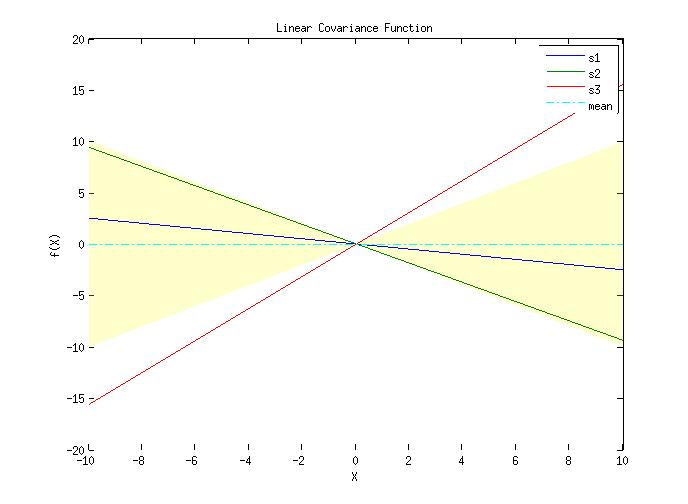
\includegraphics[width=0.8\textwidth]{1_a_1.jpg}
\caption{Linear Covariance Function}
\label{fig:1a1}
\end{figure}
\begin{figure}[H]
\centering
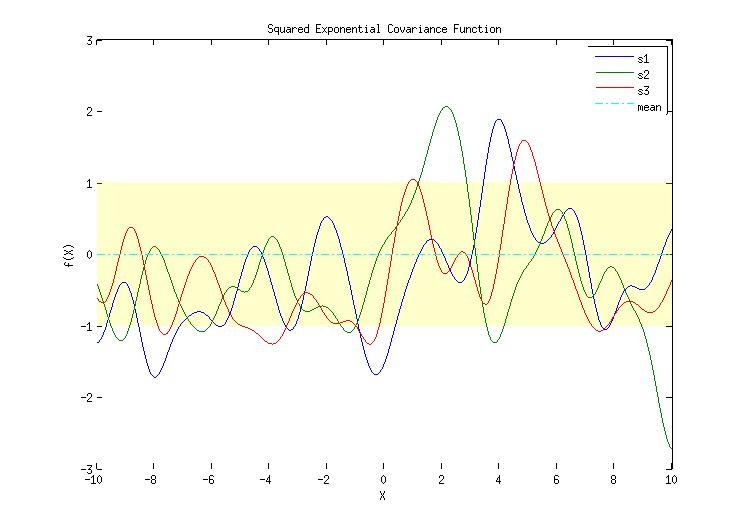
\includegraphics[width=0.8\textwidth]{1_a_2.jpg}
\caption{Square Exponential Covariance Function}
\label{fig:1a2}
\end{figure}
\begin{figure}[H]
\centering
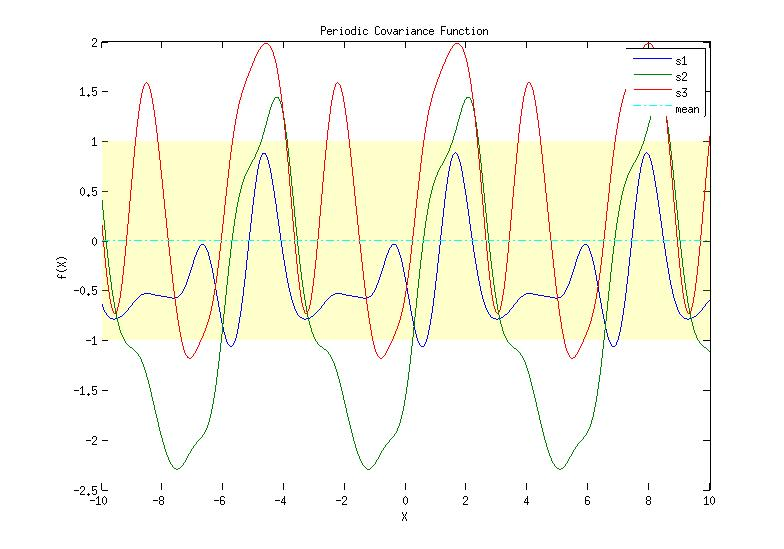
\includegraphics[width=0.8\textwidth]{1_a_3.jpg}
\caption{Periodic Covariance Function}
\label{fig:1a3}
\end{figure}

\item Increasing $\sigma^2$ increases the ``noisyness" of the output points, $y_i$.
Figure~\ref{fig:1b} shows... TODO

\begin{figure}[H]
\centering
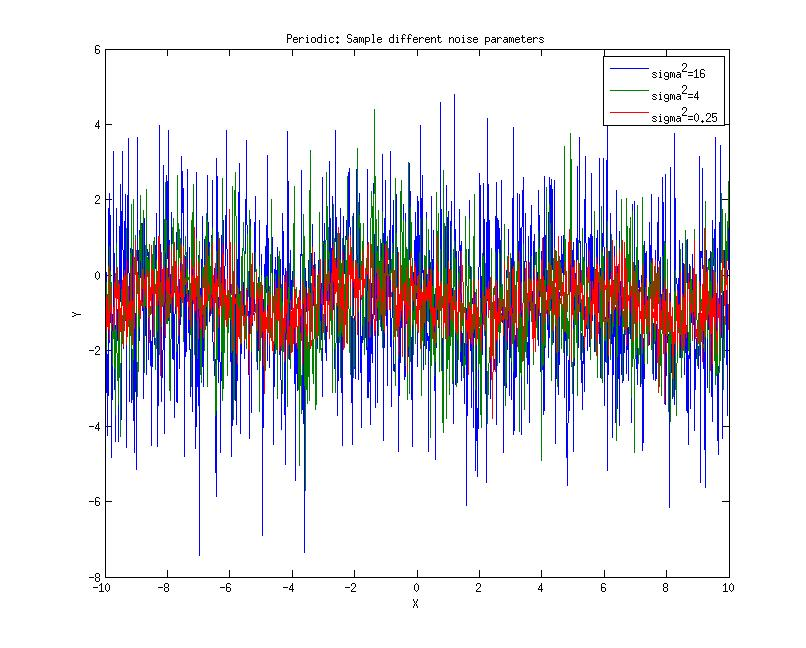
\includegraphics[width=0.8\textwidth]{1_b.jpg}
\caption{Sampling Different Gaussian Noise Parameters Using a Periodic Covariance Function}
\label{fig:1b}
\end{figure}

\item Show $p(x_1|x_2)\propto{}p(x_1,x_2)$ \\

\begin{equation*}
p(X_1|x_2)=\frac{1}{sqrt{(2\pi)^k}|\Sigma_{x_1|x_2}|}exp\Big(-\frac{1}{2}(x-\mu_{x_1|x_2})\Big)
\end{equation*}

\[
\begin{bmatrix}
  x_1 \\ x_2
\end{bmatrix}
\sim{}N \Bigg(
\begin{bmatrix}
  \mu_1 \\ \mu_2
\end{bmatrix}
\begin{bmatrix}
  \Sigma_{11} & \Sigma{12} \\ \Sigma{21} & \Sigma{22}
\end{bmatrix}
\Bigg)
\]

Let $\Sigma^{-1}=\Lambda^{-1}$ such that
\[
\Sigma^{-1}=
\begin{bmatrix}
  \Sigma_{11} & \Sigma_{12} \\ \Sigma_{21} & \Sigma_{22}
\end{bmatrix}
^{-1}=
\begin{bmatrix}
  \Lambda_{11} & \Lambda_{12} \\ \Lambda_{21} & \Lambda_{22}
\end{bmatrix}
=\Lambda
\]

We can focus on the exponent since we want to find $\mu_{x_1|x_2}$ and $\Sigma_{x_1|x_2}$.

%\begin{equation}
%\begin{align*}
%-\frac{1}{2}(x-\mu)^T\Sigma^{-1}(x-\mu) 
%&=-\frac{1}{2}(x-\mu)^T\Sigma^{-1}(x-\mu) 
%\end{align*}
%\end{equation}

\begin{align*}
exp&=-\frac{1}{2}(x-\mu)^T\Sigma^{-1}(x-\mu) \\
&=-\frac{1}{2}
\begin{bmatrix}
  x_1 - \mu_1 \\ x_2 - \mu_2
\end{bmatrix}
^T
\begin{bmatrix}
  \Sigma_{11} & \Sigma_{12} \\ \Sigma_{21} & \Sigma_{22}
\end{bmatrix}
^{-1}
\begin{bmatrix}
  x_1 - \mu_1 \\ x_2 - \mu_2
\end{bmatrix} \\
&=-\frac{1}{2}
\begin{bmatrix}
  x_1 - \mu_1 \\ x_2 - \mu_2
\end{bmatrix}
^T
\begin{bmatrix}
  \Lambda_{11} & \Lambda_{12} \\ \Lambda_{21} & \Lambda_{22}
\end{bmatrix}
\begin{bmatrix}
  x_1 - \mu_1 \\ x_2 - \mu_2
\end{bmatrix}
\end{align*}

\begin{multline*}
=-\frac{1}{2}(x_1-\mu_1)^T\Lambda_{11}(x_1-\mu_1)
-\frac{1}{2}(x_1-\mu_1)^T\Lambda_{12}(x_2-\mu_2) \\
-\frac{1}{2}(x_2-\mu_2)^T\Lambda_{21}(x_1-\mu_1) 
-\frac{1}{2}(x_2-\mu_2)^T\Lambda_{22}(x_2-\mu_2)
\end{multline*}

We can call the last term, $-\frac{1}{2}(x_2-\mu_2)^T\Lambda_{22}(x_2-\mu_2)$, $C$ since it does not depend on $x_1$ (constant).

\begin{multline*}
=-\frac{1}{2}(x_1-\mu_1)^T\Lambda_{11}(x_1-\mu_1)
-\frac{1}{2}(x_1-\mu_1)^T\Lambda_{12}(x_2-\mu_2)
-\frac{1}{2}(x_2-\mu_2)^T\Lambda_{21}(x_1-\mu_1) 
+C
\end{multline*}

\begin{multline*}
=-\frac{1}{2}x_1^T\Lambda_{11}x_1
+\frac{1}{2}x_1^T\Lambda_{11}\mu_1
+\frac{1}{2}\mu_1^T\Lambda_{11}x_1
-\frac{1}{2}\mu_1^T\Lambda_{11}\mu_1 \\
-\frac{1}{2}x_1^T\Lambda_{12}x_2
+\frac{1}{2}x_1^T\Lambda_{12}\mu_2
+\frac{1}{2}\mu_1^T\Lambda_{12}x_2
-\frac{1}{2}\mu_1^T\Lambda_{12}\mu_2 \\
-\frac{1}{2}x_2^T\Lambda_{21}x_1
+\frac{1}{2}x_2^T\Lambda_{21}\mu_1
+\frac{1}{2}\mu_2^T\Lambda_{21}x_1
-\frac{1}{2}\mu_2^T\Lambda_{21}\mu_1+C
\end{multline*}

Again, include any constants that do not depend on $x_1$ in C.

\begin{multline*}
=-\frac{1}{2}x_1^T\Lambda_{11}x_1
+\frac{1}{2}x_1^T\Lambda_{11}\mu_1
+\frac{1}{2}\mu_1^T\Lambda_{11}x_1
-\frac{1}{2}x_1^T\Lambda_{12}x_2
+\frac{1}{2}x_1^T\Lambda_{12}\mu_2
-\frac{1}{2}x_2^T\Lambda_{21}x_1
+\frac{1}{2}\mu_2^T\Lambda_{21}x_1+C
\end{multline*}

We can use the fact that $\Lambda_{21}=\Lambda_{12}^T$ to reduce the equation.

\begin{equation*}
=-\frac{1}{2}x_1^T\Lambda_{11}x_1
+x_1^T\Lambda_{11}\mu_1
-x_1^T\Lambda_{12}x_2
+x_1^T\Lambda_{12}\mu_2+C
\end{equation*}



\item % (d)

\item A comparison of covariance functions sampled from $p(f(X)|Y_\ast)$: see figures~\ref{fig:1e1},~\ref{fig:1e2}, and~\ref{fig:1e3}.

\begin{figure}[H]
\centering
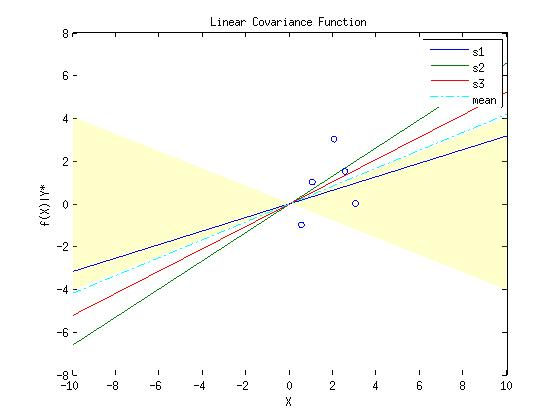
\includegraphics[width=0.8\textwidth]{1_e_1.jpg}
\caption{Linear Covariance Function}
\label{fig:1e1}
\end{figure}
\begin{figure}[H]
\centering
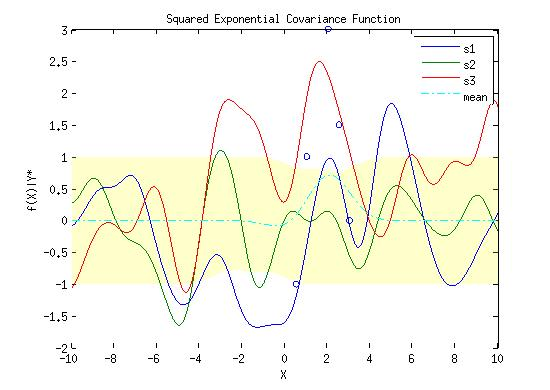
\includegraphics[width=0.8\textwidth]{1_e_2.jpg}
\caption{Square Exponential Covariance Function}
\label{fig:1e2}
\end{figure}
\begin{figure}[H]
\centering
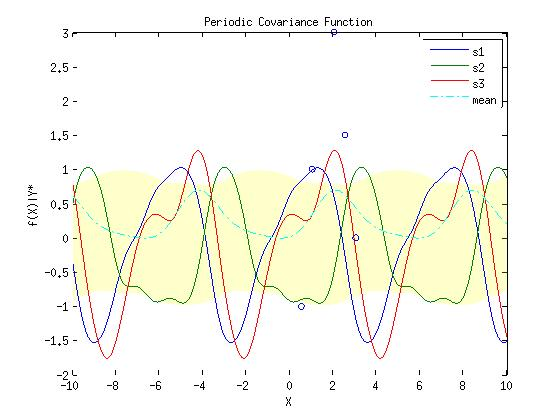
\includegraphics[width=0.8\textwidth]{1_e_3.jpg}
\caption{Periodic Covariance Function}
\label{fig:1e3}
\end{figure}

\item TODO

\begin{figure}[H]
\centering
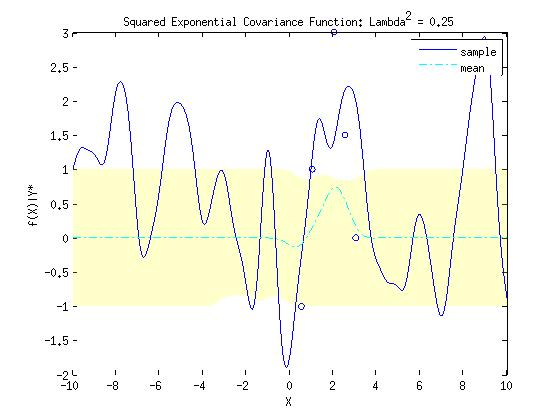
\includegraphics[width=0.8\textwidth]{1_f_1.jpg}
\caption{Sampling Different $\lambda^2$ Parameters Using the Squared Exponential Function}
\label{fig:1f1}
\end{figure}

\begin{figure}[H]
\centering
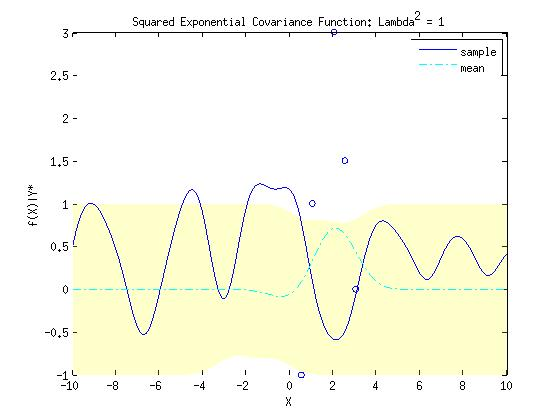
\includegraphics[width=0.8\textwidth]{1_f_2.jpg}
\caption{Sampling Different $\lambda^2$ Parameters Using the Squared Exponential Function}
\label{fig:1f2}
\end{figure}

\begin{figure}[H]
\centering
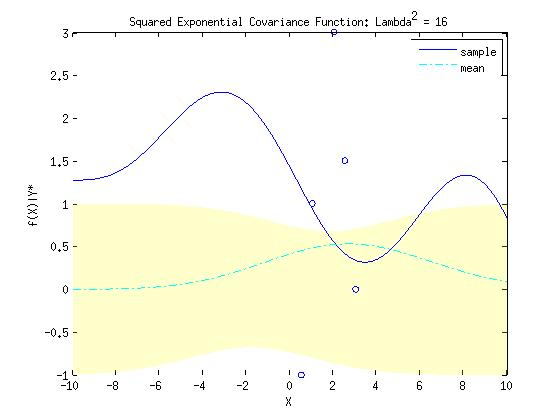
\includegraphics[width=0.8\textwidth]{1_f_3.jpg}
\caption{Sampling Different $\lambda^2$ Parameters Using the Squared Exponential Function}
\label{fig:1f3}
\end{figure}

\end{enumerate}
\end{document}
\documentclass{article}
\usepackage{bm}
\usepackage{amsmath}
\usepackage{amssymb}
\usepackage{graphicx}
\usepackage[colorlinks=true,urlcolor=blue]{hyperref}
\usepackage{geometry}
\geometry{margin=1in}
\usepackage{multicol}
\usepackage{paralist}
\usepackage{todonotes}
\setlength{\marginparwidth}{2.15cm}
\usepackage{booktabs}
\usepackage{enumitem}
\graphicspath{{../}}
\usepackage{setspace}
\doublespacing

\newcommand{\norm}[1]{\left\lVert#1\right\rVert}

\begin{document}

\section*{}
\begin{center}
  \centerline{\textsc{\LARGE Homework 3}}
  \vspace{0.5em}
  \centerline{\textsc{Regression, Gaussian Processes, and Boosting}}
  \vspace{1em}
  \textsc{\large Dana Van Aken} \\
\end{center}

\section*{Problem 1: Gaussian Processes}

\begin{enumerate}[label=(\alph*)]
\setlength\itemsep{1em}

\item % (a)

\item % (b)

\item % (c)

\item % (d)

\item % (e)

\item % (f)

\end{enumerate}

\section*{Problem 2: Regression}

\subsection*{2.1 Why Lasso Works}

\begin{enumerate}
\setlength\itemsep{1em}

\item Write $J_\lambda(\beta)$ in the form $J_\lambda(\beta)=g(y)+\sum_1^df(X_i,y,\beta_i,\lambda)$, $\lambda > 0$: 

$J_\lambda(\beta)=\frac{1}{2}\norm{y-X\beta}^2+\lambda\norm{\beta}$ 

$=\frac{1}{2}(y-X\beta)^T(y-X\beta)+\lambda\norm{\beta}$ 

$=\frac{1}{2}[y^Ty-2y^TX\beta+(X\beta)^TX\beta]+\lambda\norm{\beta}$ 

$=\frac{1}{2}[y^Ty-2y^TX\beta+\beta^TX^TX\beta]+\lambda\norm{\beta}$ 

$=\frac{1}{2}[y^Ty-2y^TX\beta+\beta^T\beta]+\lambda\norm{\beta}$ \hfill $(X^TX=I)$ 

$=\frac{1}{2}y^Ty-y^TX\beta+\frac{1}{2}\beta^T\beta+\lambda\norm{\beta}$ 

$=\frac{1}{2}y^Ty+\sum_{i=1}^d\frac{1}{2}\beta_i^T\beta_i-y^TX_i\beta_i+\lambda\norm{\beta_i}$ 

Let $g(y)=\frac{1}{2}y^Ty$ and $f(X_i,y,\beta_i,\lambda)=\frac{1}{2}\beta_i^T\beta_i-y^TX_i\beta_i+\lambda\norm{\beta_i}$, then: 

$\bm{J_\lambda(\beta)=g(y)+\sum_{i=1}^df(X_i,y,\beta_i,\lambda)}$ 



\item $\beta_i^\ast>0$:

Calculating the derivative of $f(X_i,y,\beta_i^\ast,\lambda)$, (where $i$ in $\{1...d\}$), we get: 

$\frac{f(X_i,y,\beta_i^\ast,\lambda)}{d\beta_i^\ast}=\beta_i^\ast-y^TX_i+\lambda$

Setting the LHS equal to zero and solving for $\beta_i^\ast$ gives:

\begin{equation}
\bm{\beta_i^\ast=y^TX_i-\lambda}
\end{equation}


\item $\beta_i^\ast<0$:

Calculating the derivative of $f(X_i,y,\beta_i^\ast,\lambda)$, (where $i$ in $\{1...d\}$), we get: 

$\frac{f(X_i,y,\beta_i^\ast,\lambda)}{d\beta_i^\ast}=-\beta_i^\ast-y^TX_i+\lambda$

Setting the LHS equal to zero and solving for $\beta_i^\ast$ gives:

\begin{equation}
\bm{\beta_i^\ast=-y^TX_i+\lambda}
\end{equation}

\item % (4)

In both equations (1) and (2), as we increase $\lambda$, $\beta_i^\ast$ gets closer and closer to zero
(assuming $\beta_i^\ast$ and $y^TX_i$ are the same sign).
Once you increase $\lambda$ enough that $\beta_i^\ast$ reaches zero, it sticks there because moving it below zero
increases the L1 penalty and moves it further away from the least squares term (mathematically, $\lambda$ switches
its sign at this point because of the characteristics of the absolute value function). 

\item % (5)

Calculating the derivative of $f(X_i,y,\beta_i^\ast,\lambda)$, (where $i$ in $\{1...d\}$),
with the regularization term $\frac{1}{2}\norm{\beta_i^\ast}_2^2$ we get: 

$\frac{f(X_i,y,\beta_i^\ast,\lambda)}{d\beta_i^\ast}=\beta_i^\ast-y^TX_i+\lambda\beta_i^\ast$

Setting the LHS equal to zero and solving for $\beta_i^\ast$ gives:

$\beta_i^\ast=\frac{y^TX_i}{1+\lambda}$

Unlike equations (1) and (2), there is no value of alpha that can drive $\beta_i^\ast$ to zero.
This demonstrates why Lasso regression often results in ``sparser" solutions whereas Ridge regression
does not.

\end{enumerate}
\subsection*{2.2 Bayesian regression and Gaussian process}

\begin{enumerate}
\setlength\itemsep{1em}

\item % (1)

\begin{enumerate}

\item % (a)

\item % (b)

\end{enumerate}

\item % (2)

\item % (3)

\item % (4)

\end{enumerate}
\end{document}
\section*{Problem 3: Implementing Naive Bayes and Logistic Regression [Adona - 50 pts]}

In this question you will code two of the classification algorithms covered in class: \emph{Naive Bayes} and \emph{Logistic Regression}. Remember to follow the detailed coding and submission instructions at the top of this file!

\begin{itemize}
\item \textbf{Data:} All questions will use the following datastructures:
\begin{itemize}
\item $\mathit{XTrain} \in \mathbb{R} ^{n \times f}$ is a matrix of training data, where each row is a training point, and each column is a feature.
\item $\mathit{XTest} \in \mathbb{R} ^{m \times f}$ is a matrix of test data, where each row is a test point, and each column is a feature.
\item $\mathit{yTrain} \in \{1,...,c\}^{n \times 1} $ is a vector of training labels
\item $\mathit{yTest} \in \{1,...,c\}^{m \times 1} $ is a (hidden) vector of test labels. 
\end{itemize}  


\item \textbf{SUBMISSION CHECKLIST}
\begin{itemize}
\item Submission executes on our machines in less than 20 minutes.
\item Submission is smaller than 1MB.
\item Submission is a \verb#.tar# file.
\item Submission returns matrices of the \emph{exact} dimension specified.
\end{itemize}
\end{itemize}

\newpage
\subsection*{Logspace Arithmetic [7 pts]}

When working with very small and very large numbers (such as probabilities), it is useful to work in \emph{logspace} to avoid numerical precision issues. In logspace, we keep track of the logs of numbers, instead of the numbers themselves. (We generally use natural logs for this). For example, if $p(x)$ and $p(y)$ are probability values, instead of storing $p(x)$ and $p(y)$ and computing $p(x)*p(y)$, we work in log space by storing $\log p(x), \log p(y), \log [p(x)*p(y)]$, where $\log [p(x)*p(y)]$ is computed as $\log p(x)+\log p(y)$.

The challenge is to add and multiply these numbers \emph{while remaining in logspace}, without exponentiating. Note that if we exponentiate our numbers at any point in the calculation it completely defeats the purpose of working in log space. Hint: Alex Smola has an excellent \href{http://blog.smola.org/post/987977550/log-probabilities-semirings-and-floating-point-numbers}{post} on his blog about this topic.
\begin{enumerate}
\item \textbf{Logspace Multiplication [2 pts]}\\
Complete the function \textsf{logProd(x)} which takes as input a vector of numbers in logspace (i.e., $x_i = \log p_i$), and returns the product of these numbers in logspace -- i.e., \textsf{logProd(x)} $= \log \prod_i p_i$.
\item \textbf{Logspace Addition [5 pts]}\\
Complete the function \textsf{logSum(x)} which takes as input a vector of numbers in logspace (i.e., $x_i = \log p_i$), and returns the sum of these numbers in logspace -- i.e., \textsf{logSum(x)} $= \log \sum_i p_i$.
\end{enumerate}

\subsection*{Naive Bayes [12 pts]}
The dataset for this question can be downloaded at \url{https://autolab.cs.cmu.edu/10701-f14/attachments/view/230}. This is a real dataset called \emph{Iris} from the \href{http://archive.ics.uci.edu/ml/datasets/iris}{UCI machine learning repository}.

In this question you will implement the Gaussian Naive Bayes Classification algorithm. As a reminder, in the Naive Bayes algorithm we calculate $p(c|f) \propto p(f|c)p(c) = p(c) \prod_i p(f_i|c)$. In Gaussian Naive Bayes we learn a one-dimensional Gaussian for each feature in each class, i.e. $p(f_i|c) = N(f_i; \mu_{i,c},\sigma^2_{i,c})$, where $\mu_{i,c}$ is the mean of feature $f_i$ for those instances in class $c$, and $\sigma^2_{i,c}$ is the variance of feature $f_i$ for instances in class $c$. You can (and should) test your implementation locally using the $\mathit{XTrainIris}$ and $\mathit{yTrainIris}$ data provided.
\begin{enumerate}
\item \textbf{Prior [2 pts]}\\
Complete the function \textsf{[p] = NBprior(yTrain)}. $p$ is a $c \times 1$ vector where $p_i$ is the prior probability of class $i$.
\item \textbf{Parameter Learning [5 pts]}\\
Complete the function \textsf{[M,V] = NBparameters(XTrain, yTrain)}. $M$ is an $c \times f$ matrix where $M_{i,j}$ is the conditional mean of feature $j$ given class $i$. $V$ is an $c \times f$ matrix where $V_{i,j}$ is the conditional variance of feature $j$ given class $i$.
\item \textbf{Naive Bayes Classifier [5 pts]}\\
Complete the function \textsf{[t] = NBclassify(XTrain, XTest, yTrain)}. $t$ is a $m \times 1$ vector of predicted class values, where $t_i$ is the predicted class for the $i$th row of $\mathit{XTest}$.
\end{enumerate}

\subsection*{Binary Logistic Regression [17 pts]}

In the following two problems, we will implement Binary and Multi-class Logistic Regression. Although Multi-class LR is a direct generalization of the binary case, the two algorithms are often formalized slightly differently (e.g. the two binary case only has one vector $w \in f \times 1$ while the equivalent "multi-class" binary implementation has a matrix $W in 2 \times f$). The two formulations are equivalent, but each is more natural to manipulate in its specific context. Binary LR is slightly easier to derive and implement, so we will start here. As you progress to Multi-class LR, try to notice the parallels - this will minimize work and maximize intuition :).

\textbf{NOTE:} If you're feeling adventurous, you can instead start by directly implementing multi-class LR. However, you will then have to write a wrapper function for each binary method converting between the two representations (e.g. converting $W$ to $w$). This should be less work if you're experience with ML, but is not recommended if this is your first time implementing these algorithms. \\

The dataset for this question can be downloaded at \url{https://autolab.cs.cmu.edu/10701-f14/attachments/view/230}. This is another real dataset called the \textit{Wisconsin Breast Cancer Database}, also from \href{http://archive.ics.uci.edu/ml/datasets/Breast+Cancer+Wisconsin+%28Original%29}{UCI}. \\

You will train the Logistic Regression Classifier using numerical optimization of the Maximum Likelihood Estimator (MLE). Since we haven't covered numerical optimization techniques in class yet, we have provided you with helper code, implementing a very rudimentary version of gradient descent. Feel free to check it out! 


\begin{enumerate}
\item \textbf{Sigmoid Probability [2 pts]}\\
Complete the function \textsf{[p] = LRprob(x, w)}. $x$ is a single training example ($1 \times f$), $w$ is a $f \times 1$ weights vector, and $p = p(y|x)$ is a $2 \times 1$ vector of class probabilities.

\item \textbf{Conditional Log Likelihood [5pts]}\\
Complete the function \textsf{[logl] = LRlogLikelihood(X, y, w)}. $logl$ is the scalar conditional log likelihood of the data, $(y|X)$, under the model with parameters $w$.

\item \textbf{Gradient of the Conditional Log Likelihood [5pts]}\\
Complete the function \textsf{[grad] = LRgradient(X, y, w)}. $grad$ is a $f \times 1$ vector representing the gradient of the conditional log likelihood with respect to $w$. 

\item \textbf{Logistic Regression Classifier [5pts]}\\
Complete the function \textsf{[cls] = LRclassify(XTrain, yTrain, XTest)}. $cls$ is a $m \times 1$ vector representing the predicted test class labels. 
\end{enumerate}

\subsection*{Multiclass Logistic Regression [14 pts]}
To test the MultiClass LR Classifier we will again use the \textit{Iris} dataset we used for Naive Bayes above. As always, you can and should test your implementation locally using $XTrainIris$ and $YTrainIris$ data provided. 

\begin{enumerate}
\item \textbf{Probability [2 pts]}\\
Complete the function \textsf{[p] = mLRprob(x, W)}. $x$ is a single training example ($1 \times f$), $W$ is a $c \times f$ weights \textit{matrix} where each row $c$ is the weights vector $w_c$, and $p = p(y|x)$ is a $c \times 1$ vector of class probabilities.

\item \textbf{Conditional Log Likelihood [4pts]}\\
Complete the function \textsf{[logl] = mLRlogLikelihood(X, y, W)}. As before, $logl$ is the scalar conditional log likelihood of the data, $(y|X)$, under the model with parameters $W$.

\item \textbf{Gradient of the Conditional Log Likelihood [4pts]}\\
Complete the function \textsf{[grad] = mLRgradient(X, y, W)}. $grad$ is a $c \times f$ \textit{matrix} representing the gradient of the conditional log likelihood with respect to $W$. 

\item \textbf{Logistic Regression Classifier [4pts]}\\
Complete the function \textsf{[cls] = mLRclassify(XTrain, yTrain, XTest)}. As before, $cls$ is a $m \times 1$ vector representing the predicted test class labels. 
\end{enumerate}



\end{document}
